\chapter{Electronic mail processing}
\label{mailprocess}
E-mail or Electronic mail is a mean for sending and receiving messages between two users on the internet. To process an e-mail, it is necessary to understand the format of e-mail message as defined by multiple RFCs (Request for Comments). Generally, an e-mail is a text document separated into a header and a body. The header contains meta-information about the e-mail, the body contains the actual message. Encoding of the messages is further explained in the 
\autoref{mime}.

This chapter describes the important parts of the format for the processing of an e-mail message as defined by RFC 5322~\cite{rfc5322}, the protocols that define the e-mail communication (SMTP, IMAP and POP), and the transfer agents that make use of these protocols and ensure the communication.

\section{History}
First use of electronic messages as a form of communication can be traced back to early 1960s\footnote{\texttt{http://www.nethistory.info/History\%20of\%20the\%20Internet/email.html}}. Using the Compatible Time-Sharing System, hundreds of users at the MIT Computation Center could log into the remote dial-up terminals to store their files.
This way of sharing data encouraged new ways of communication to be invented. The \texttt{mail} command for the CTSS was written in the 1965 to work with e-mail within a single computer.

Ray Tomlinson is considered to be the creator of the e-mail: He was the first one to use the symbol @ for denoting a message to be sent between the computers on ARPANET in 1972. Since then, ARPANET encouraged the usage of e-mails which quickly became widespread. Soon after, the protocols and tools for the foldering and e-mail organization were invented.

Historically, one of the most important e-mail standards is \emph{Simple Message Transfer Protocol} (\emph{SMTP}), defined in the 1982. Starting as a complement to the already existing \emph{Unix to Unix Copy Program} (\emph{UUCP}), SMTP soon started to be widely used. Nowadays, majority of the e-mail communication is done via SMTP.  Nevertheless, the protocol is designed only for the message-pushing transfers. Additional protocols are required to support other use-cases.

\emph{Post Office Protocol} (shortly \emph{POP}) appeared in the 1984. It was an important standard as it stated the rules of an e-mail message retrieval to personal computers, which consequently helped to standardize the communication between the user and the mail server. Nowadays, the most used internet protocols for e-mail communication are POP3, IMAP and SMTP, further discussed in \autoref{smtp} and \autoref{popimap}.

\section{Message Format}
Multiple standards defining the e-mail message format were created throughout the years. Probably the most important one was defined by RFC 822, as it was the first protocol standardizing the e-mail message format. 20 years after being published, it was replaced by RFC 2822 in the 2005 which was later obsoleted in the 2008 by RFC 5322.
The following sections summarize the current e-mail format standard, defined by RFC 5322~\cite{rfc5322}.

E-mail message, as defined by RFC 5322, is split into two major parts, the \emph{header} and the \emph{body}.

\subsection{Header}
The \emph{header} is composed of \emph{fields} that contain meta-information about the e-mail (e.g. subject of the message, sender of the message\dots).
Field is a pair of two text values separated by a colon:
\begin{center}
\texttt{field name: field value}
\end{center}
If a line in the header begins with 7-bit ASCII character, it is a field. If a line starts with white space, the value of the field from the previous line continues on the current line, which makes multi-line fields possible. The values of the fields have to be 7-bit ASCII as well. To encode a non-ASCII value of a field, \emph{MIME} encoding is used. 

\label{mime}
\emph{MIME} is a standard that describes the encoding of non-ASCII values to 7-bit ASCII (e.g. to support multiple different charsets or structured values). To encode a string in a different charset, the following syntax is used:
\begin{center}
\texttt{=?charset?encoding?encoded text?=}
\end{center}
For example:
\begin{center}
\texttt{=?iso-8859-1?Q?=A1Hola,\_se=F1or!?=}
\end{center}
After decoding the encoded text using the provided charset and the encoding, we obtain the value \texttt{¡Hola, señor!}. A typical use of the MIME encoding is the support for different languages.

Only two header fields are mandatory for each message: \texttt{Date} and \texttt{From}. All other fields are optional, however, there are several fields that are recommended and several fields that are commonly used. Most of these fields are described in \autoref{table:fields}. 
\begin{table}[t]
\centering
\renewcommand{\arraystretch}{1.4}
\begin{tabular}{l p{20em}}
 \toprule
 Field name & Description\\
\midrule
 \texttt{Date} & Date of origination (mandatory)\\
 \texttt{From} & Address of the sender (mandatory)\\
 \texttt{Message-ID} & Recommended for the message identification\\
 \texttt{In-Reply-To} & Recommended, if the message is a reply\\
 \texttt{References} & Recommended, if the message references to other messages\\
 \texttt{Sender} & Displayed sender (optional)\\
 \texttt{Reply-To} & The address to reply (optional)\\
 \texttt{To} & Displayed recipient (optional)\\
 \texttt{Cc} & Carbon Copy, used for sending copies of e-mail to multiple users (optional)\\
 \texttt{Bcc} & Blind Carbon Copy, same as Cc except the recipients are not visible (optional)\\
 \texttt{Subject} & Subject of the message (optional)\\
 \texttt{Return-Path} & Return address (optional)\\
\bottomrule
\end{tabular}
\caption{Header fields as defined by RFC 5322.}
\label{table:fields}
\end{table}
A detail worth mentioning is that the \texttt{To} and \texttt{From} fields do not have to necessarily be the same addresses as the actual sender and recipient addresses. These fields are just informative, the real addresses are given to the SMTP for the mail delivery. SMTP is described further in \autoref{smtp}. 

An example of headers of a real e-mail message is displayed in \autoref{fig:message}.
\begin{figure}
\centering
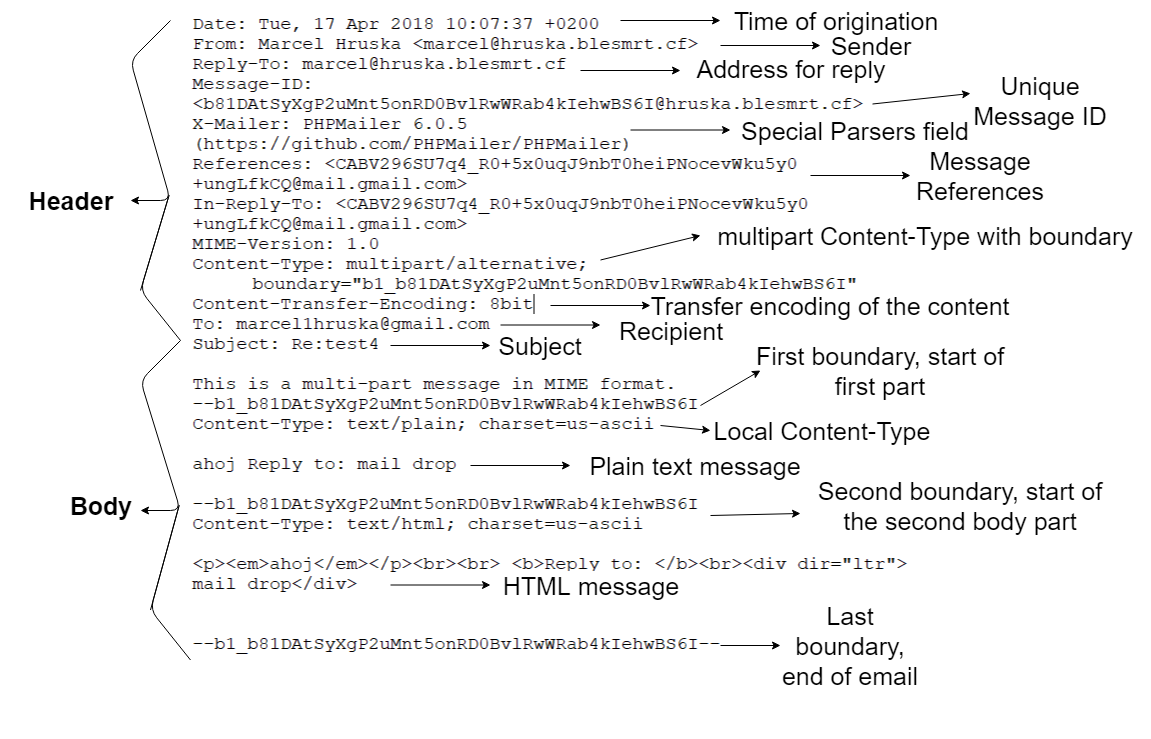
\includegraphics[width=\textwidth]{img/message_example.png}
\caption{A message sent from KamehaMail to a user of Gmail.}
\label{fig:message}
\end{figure}

\subsection{Body}
This section describes the format of the content of the message, called body.
RFC 5322 does not describe an exact format of message body, but references other documents for this purpose. For example, RFC 2045~\cite{rfc2045} from 1996 describes how the body of the message is supposed to look (its format, syntax\dots). We cover only the parts of RFC 2045 necessary for the purposes of this thesis.
The body is separated from the header by one blank line.

Originally, the messages were meant to be plain-text 7-bit ASCII only. However, it is possible to use the MIME encoding for the message bodies as well. 

If the user decides to use the MIME encoding for the message body, three header fields must be filled in: \texttt{MIME-Version}, \texttt{Content-Type} and \texttt{Content-Transfer-Encoding}.

\texttt{MIME-Version} is the version of the MIME being used for the encoding of the message, currently \texttt{1.0}.

\texttt{Content-Transfer-Encoding} specifies the encoding of the body. For example, SMTP expects messages to be 7-bit US-ASCII, which can be changed to 8-bit encoding using this header, making successive encoding more convenient.

\texttt{Content-Type} describes the type of data so that the receiving part understands how to decode the contents of the e-mail properly. This value is called \emph{media type}. Each media type has its subtype identifier, which further refines the media type. After the type identifiers comes a semicolon and parameters, if necessary. For example,
\begin{center}
\texttt{Content-type: text/plain; charset="us-ascii"}
\end{center}
defines media type \texttt{text}, its subtype \texttt{plain} and the parameter defining the charset \texttt{charset="us-ascii"}. This is also the default value, if the header is not present.

\subsubsection{Multipart messages}
There is a commonly used media type that we want to mention specifically, described by RFC 1341~\cite{rfc1341}, called \emph{multipart}.
The multipart content-type allows to combine multiple bodies/body parts in a single message, each possibly encoded in a different way. Vast majority of the modern e-mail clients uses it to send two bodies: an HTML body for the user interfaces that are capable of displaying HTML messages, and a plain-text body for the compatibility with simple plain-text interfaces.
Another widespread use of the multipart media type is to encode the attachments into the body of the e-mail.

All subtypes of the multipart content-type follow the same syntax. The header must specify a parameter called \emph{boundary}, which is used to separate the body parts by two hyphens and the boundary string. Each of the separated body parts has its own content-type header defining its inner message type. The syntax of multipart content-type is displayed in the example in \autoref{fig:message}.

\section{Message exchange}
Because it is too complicated to send a message directly to end recipient's computer with knowing only his e-mail address, a more complicated infrastructure is used for e-mail delivery. 
The computers in this infrastructure are classified by the role they have as \emph{Mail Transfer agents} (MTA), \emph{Mail User Agents} (MUA), \emph{Mail Delivery Agents} (MDA) and \emph{Mail Submission Agents} (MSA).

This section gives a closer description of the roles of e-mail agents and the communication protocols that the e-mail agents use.

\subsection{E-mail Agents}
The end-to-end delivery of a message has several stages: the submission of the message, the transfer of the message and the retrieval. Many complications can occur during the transport, such as non-existing final destination or disconnected user. \emph{E-mail agents} were invented to take care of these situations which are futher detailed in the following sections as defined by RFC 5598~\cite{rfc5598}.

\subsubsection{Mail Transfer Agent}
\emph{Mail Transfer Agent} (also known as \emph{Mail Server}) is designed to transfer e-mail messages, implementing both sending and receiving parts of the SMTP protocol.
It is often called a mail relay as well because its job is to route and forward e-mails to their final destinations.

MTAs are running in the background. They are listening to a port, waiting for the message to come, either from another MTA or from the user. If the message comes from another MTA, it is either routed to the next MTA on its path or in case that the current MTA is its final destination, stored locally for the user. 
UNIX mail servers exim, postfix or sendmail are all examples of MTAs.

MTA does not implement the access to the messages for the user, which needs to be handled by different agents.

\subsubsection{MUA, MSA, MDA}
For the communication between the user and the MTA, \emph{Mail User Agent} (also known as \emph{e-mail client}) is used. MUA 's main role is to retrieve e-mails from the MTA for the user and display them. It often implements the interface for the composition of an e-mail. E-mails created by an e-mail client are then sent to the corresponding MTA for distribution.
Usually, the communication between MUA and MTA is not direct. Two more systems are commonly used as a layer between MUA and MTA: \emph{Mail Submission Agent} and \emph{Mail Delivery Agent}.

MSA takes care of the submission of a message from MUA to MTA. It uses SMTP as well but listens to a different port. Some of the advantages of having an MSA are the following: It enforces the policies of the standard protocols while representing the interests of the author of the message. It rejects messages that do not satisfy the conditions stated by the internet standards. It includes header fields such as \texttt{Date} or \texttt{Message-ID}. In some cases, it can help to solve minor errors.

MDA takes responsibility of storing an e-mail for the user from MTA and delivers the message to the recipient's MUA. Common role of the MDA is to redirect the message to user-defined address. 

A simple diagram of the e-mail flow is shown in the \autoref{fig:mail-flow}.
 \begin{figure}
\centering
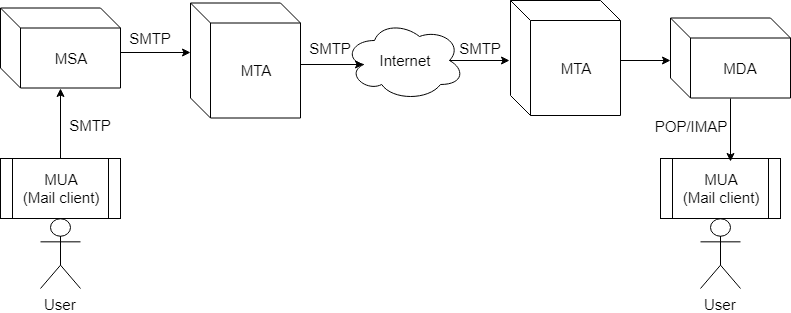
\includegraphics[width=\textwidth]{img/mail_flow.png}
\caption{A simple diagram of the e-mail transfer flow between two users.}
\label{fig:mail-flow}
\end{figure}
The transfer of the messages between two MTAs is defined by SMTP. The retrieval of the message to the MUA is done using IMAP or POP.

\subsection{E-mail protocols}
\subsubsection{SMTP}
\label{smtp}
In the previous sections, we mentioned the internet protocol SMTP which is a standard for an e-mail transfer. It was first defined in the 1982 by RFC 821~\cite{rfc821} and last updated in the 2008 by RFC 5321.
SMTP defines a model of communication as follows: The user sends a request to the sender-SMTP\footnote{sender-SMTP and receiver-SMTP are servers capable of communicating via SMTP, usually MTA} to start an e-mail communication. The sender-SMTP opens a two-way communication with the corresponding receiver-SMTP which is either an intermediate or the final destination. After that, the user can submit mail commands via the established communication path and receive the responses.
The \autoref{fig:smtp-model} shows the SMTP model as described by RFC 821.
\begin{figure}
\centering
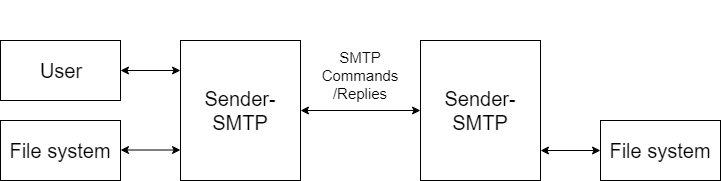
\includegraphics[width=\textwidth]{img/smtp_model.png}
\caption{Model for SMTP use.}
\label{fig:smtp-model}
\end{figure}

To begin an e-mail transaction, user introduces himself using \texttt{HELO} command. Then there are three stages of the SMTP mail transaction.
\begin{enumerate}
\item The first part is the \texttt{MAIL} command. This command indicates the beginning of a new e-mail transaction for the receiver-SMTP. The receiver-SMTP resets all the state data it has and prepares for the following commands corresponding to the new transaction.
\begin{center}
\texttt{MAIL <SP> FROM:<reverse-path> <CRLF>}
\end{center}
Tags \texttt{SP} and \texttt{CRLF} mean space and an end-of-line respectively. The \texttt{reverse-path} in the field \texttt{FROM} contains address where the responses will be sent, for example errors. If the command was processed successfully, the response \texttt{250 OK} is sent to the return address.
\item The second part is the \texttt{RCPT} command which defines the receiving address of the current mail transaction. 
\begin{center}
\texttt{RCPT <SP> FROM:<forward-path> <CRLF>}
\end{center}
The \texttt{forward-path} contains the address of the recipient. If the receiver-SMTP does not recognize the address, it responds with \texttt{550 Failure}. This command can be repeated for multiple recipients. If accepted, the \texttt{250 OK} reply is sent.
\item The third and the last part is the \texttt{DATA} command. This command transfers the actual data of the message.
\begin{center}
\texttt{DATA <CRLF>}
\end{center}
If the command is accepted by the receiver-SMTP, the reply \\ \texttt{354 Intermediate} \\ is sent. All following lines until the end of the text are the data of the message. The headers of the message are sent via \texttt{DATA} command as well.
\end{enumerate}
To end the transaction, the \texttt{QUIT} command is used.
The whole process is summarized in the following example~\cite{rfc821}:
\\
\texttt{S: HELO client.example.com}\\
\texttt{R: 250 Hello client.example.com}\\
\texttt{S: MAIL FROM:<Smith@Alpha.ARPA>}\\
\texttt{R: 250 OK}\\
\\
\texttt{S: RCPT TO:<Jones@Beta.ARPA>}\\
\texttt{R: 250 OK}\\
\\
\texttt{S: RCPT TO:<Green@Beta.ARPA>}\\
\texttt{R: 550 No such user here}\\
\\
\texttt{S: RCPT TO:<Brown@Beta.ARPA>}\\
\texttt{R: 250 OK}\\
\\
\texttt{S: DATA}\\
\texttt{R: 354 Start mail input; end with <CRLF>.<CRLF>}\\
\texttt{S: Blah blah blah...}\\
\texttt{S: ...etc. etc. etc.}\\
\texttt{S: <CRLF>.<CRLF>}\\
\texttt{R: 250 OK}\\
\texttt{S: QUIT}\\
\texttt{R: 221 Bye}\\
\label{mail-command}
There exists many other commands that SMTP protocol uses for the communication. However, this is all handled by MTA.

\subsubsection{POP and IMAP}
\label{popimap}
IMAP was defined by RFC 3501 in the 2003 and its current version is IMAP4~\cite{rfc3501}. POP was first specified by RFC 918 in the 1984 and its current version POP3 was defined by RFC 1939 in the 1996~\cite{rfc1939}. While they are both protocols designed for message retrieval for the e-mail client from mail server, POP is much older than IMAP.

The main difference between them is that IMAP is designed for multi-device use (tablet, phone, desktop\dots), displaying the same content on any device since the content is synchronized on the central server. POP is designed for downloading the e-mail from the mail server to the local machine without any synchronization. What's more, POP can be set to remove the messages from the server after download. In reality, both of the protocols can be setup to work in a very similar way. However, POP is unable to tell if the message was read or not or to provide meta-information about the existence of a folder.

Both provide advantages and disadvantages for the user. IMAP is more simple to set up for multi-device use as it does not create local storages of messages on every used device. However, usage of POP offers certain degree of privacy as the e-mails can be removed from the server after their download.

\section{End-user interfaces}
This section briefly describes end-user's phase of the e-mail transfer flow. An interface has to be provided for the user to interact with the mail server and retrieve or send e-mails. E-mail interfaces can be classified by the type of the interaction and the localization of the data.

\subsection{Desktop clients}
To proceed chronologically, the first e-mail clients described in this section are so-called \emph{desktop clients}. It is a common name for all clients that are installed on the user's machine and work with the messages locally, using the message retrieval protocols. They can be further subdivided into \emph{command-line} clients and clients with \emph{graphical user interface}.

\subsubsection{Command-line clients}
Historically, the first e-mails ever were sent using console commands. \emph{Com\-mand-line} clients provide only basic graphical interface for the user. We have already presented an example of SMTP \texttt{mail} command in the \autoref{mail-command}.
Although the command-line clients are an old technology, they are not extinct. On the contrary, they are still popular because of the safety reasons (no HTML and JavaScript), speed reasons (graphical interfaces take longer to load and respond) and the flexibility. For example, UNIX's \texttt{mail} command is still being frequently used.

\subsubsection{GUI clients}
As the displaying units grew bigger, e-mail clients with more advanced graphical user interfaces became popular. These are well-known by the average e-mail users as they are more user-friendly to use than the command-line clients. Some of the most popular e-mail clients are Mozilla Thunderbird or Microsoft Outlook. 

\subsection{Web based clients}
Another category of the e-mail clients are \emph{web based} clients or simply \emph{webmails}. The major difference between the desktop clients and the web based clients is that no e-mails are being downloaded locally to the user's computer. Instead, they are stored to the webserver and can be accessed by the user via web browser.
The first webmail was developed at CERN in 1993 by Hallam-Baker Phillip called The Mail Server Daemon~\cite{cern-mail}. Bigger development of the webmails began with the easier access to the Web in the 1990s an 2000s. 
However, using a web browser as an interface represents a certain level of threat because the communication over unsecured HTTP can be readable by third parties. Usage of encrypted HTTPS communication is highly recommended.
Some of the most popular webmail services are Gmail, Outlook.com and Yahoo! Mail and some of the most popular open-source webmails are squirrelmail, roundcube, rainloop, mailspring, notmuch-web\dots

\subsection{Mobile clients}
Currently, there is a new category, \emph{mobile} e-mail clients. Smart phones are incredibly popular and the mobile clients dominate e-mail client market share. Around 55\% of the e-mails were opened on mobile phones in the 2016\footnote{\texttt{https://litmus.com/blog/the-top-10-most-popular-email-clients-of-2016}}. They are very similar to the desktop clients, except that mobile clients are optimized for smaller touch screens.
